\chapter{Divisibilidade}

 Dados dois números $a, b \in \Z$, com $b \neq 0$ calculamos a divisão de $a$ por $b$ como mostra a figura abaixo:

  \begin{figure}[H]
   \centering
   \fbox{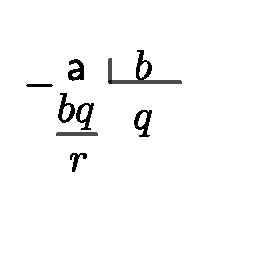
\includegraphics[width=5cm]{../Topicos/Figuras/divisao.pdf}}
   \caption{Representação conjuntos numéricos}
  \end{figure}

 logo, dados $a, b \in \Z$ existem $q, r \in \Z$ tais que $a= bq + r$.

 \vskip0.3cm

 \colorbox{azul}{
 \begin{minipage}{0.9\linewidth}
 \begin{center}
  Um número inteiro $a$ é \textbf{divisível} por um número inteiro $b$, se a divisão de $a$ por $b$ tem resto $r= 0$.
 \end{center}
 \end{minipage}}

 \vskip0.3cm

 \begin{exem}
 \begin{itemize}
 \item Todo número par é divisível por $2$.
 \item Todo número terminado em $0$ ou $5$ é divisível por $5$.
 \item Todo número divisível por $2$ e $3$ é também divisível por $6$.
 \end{itemize}
 \end{exem}

 \vskip0.3cm

 \colorbox{azul}{
 \begin{minipage}{0.9\linewidth}
 \begin{center}
  Um número $a \in \N$ diferente de $0$ e de $1$ é \textbf{primo} se for divisível apenas por $1$ e por ele mesmo.
 \end{center}
 \end{minipage}}


 \begin{exem}
 Primos: $\{2, 3, 5, 7, 11, 13, \ldots \}$
 \end{exem}

 \begin{teo}[Teorema Fundamental da Aritmética]
 Todo número $a \in \N$ diferente de $0$ e de $1$ possui uma decomposição única em números primos, em outras palavras, pode ser escrito como produto de números primos.
 \end{teo}

 \begin{defi}
 Um número $a \in \N$ diferente de $0$ e de $1$ cuja decomposição em primos possui números diferentes de $a$ é chamado de \emph{número composto}. Neste caso, $1$ e $a$ não são os únicos divisores de $a$.
 \end{defi}

 \begin{exem} De números compostos e suas fatorações em números primos:
 \begin{align*}
 &25= 5 \cdot 5 \\
 &12= 2 \cdot 2 \cdot 3 \\
 &15= 3 \cdot 5 \\
 &24= 2 \cdot 2 \cdot 2 \cdot 3
 \end{align*}
 \end{exem}

 Para ilustrar o algoritmo utilizado na fatoração dos números naturais iremos utilizá-lo para fatorar os números acima.

 \begin{tabular}{c|c}
  Números a ser fatorado & Números primos em ordem crescente \\
  25 & 5 \\
  5  & 5 \\
  1  & = 5.5  \\
 \end{tabular}

 \begin{multicols}{3}
   \begin{tabular}{c|c}
  12 & 2 \\
   6 & 2 \\
   3 & 3 \\
   1 & = 2.2.3 \\
 \end{tabular}

 \begin{tabular}{c|c}
  15 & 3 \\
   5 & 5 \\
   1 & = 3.5 \\
 \end{tabular}

 \begin{tabular}{c|c}
  24 & 2 \\
  12 & 2 \\
   6 & 2 \\
   3 & 3 \\
   1 & 2.2.2.3 \\
 \end{tabular}
 \end{multicols}

 \begin{obs}
 Um número natural sempre é divisível por todos os seus fatores primos e também pelos produtos de seus fatores primos.
 \end{obs}

 \begin{exem}
 Como $12= 2 \cdot 2 \cdot 3$, temos que seus divisores são: \[D(12)= \{1, 2, 3, 4, 6, 12\}.\]
 Como $24= 2 \cdot 2 \cdot 2 \cdot 3$, temos que seus divisores são: \[D(24)= \{1, 2, 3, 4, 6, 8, 12, 24\}.\]
 \end{exem}

 \vskip0.3cm
 \colorbox{azul}{
 \begin{minipage}{0.9\linewidth}
 \begin{center}
  \textbf{MDC - máximo divisor comum}

  Dados dois números $a, b \in \N$, o máximo divisor comum entre eles, é o maior número natural que divide $a$ e $b$. Se MDC$(a, b)= 1$ então $a$ e $b$ são primos entre si.
 \end{center}
 \end{minipage}}

 \vskip0.3cm

 \colorbox{azul}{
 \begin{minipage}{0.9\linewidth}
 \begin{center}
 \textbf{MMC - mínimo múltiplo comum}

 Dados dois números $a, b \in \N$, o mínimo múltiplo comum entre eles, é o menor número natural divisível por $a$ e $b$. Se $a$ e $b$ são primos entre si então MMC$(a, b)= ab$.
 \end{center}
 \end{minipage}}


 \begin{exem}
 \begin{align*}
 & \text{MDC}(12, 24)= 12 \\
 & \text{MMC}(12, 24)= 24
 \end{align*}
 \end{exem}

 O cálculo do MMC entre dois números pode ser feito rapidamente com auxílio de seguinte algoritmo, que apresentaremos através de exemplos:

  \begin{exem}
  \begin{enumerate}[a)]
  \item MMC(12, 24):

 \begin{tabular}{c|c}
  12, 24 & 2 \\
   6, 12 & 2 \\
   3,  6 & 2 \\
   3,  3 & 3 \\
   1,  1 &
 \end{tabular}
 $MMC(12, 24) = 2.2.2.3= 24$. Neste caso observe que 24= 2.12.

   \item MMC(9, 10):

   \begin{tabular}{c|c}
    9, 10 & 2 \\
    9, 5  & 3 \\
    3, 5  & 3 \\
    1, 5  & 5 \\
    1, 1  & \\
   \end{tabular}
   $MMC(9, 10)= 2.3.3.5= 90= 9.10$. Neste caso como 9 e 10 não possuem nenhum divisor comum, nesta situação dizemos que eles são primos entre si.

   \item MMC(12, 20):

   \begin{tabular}{c|c}
    12, 20 & 2 \\
     6, 10 & 2 \\
     3,  5 & 3 \\
     1,  5 & 5 \\
     1,  1 & \\
   \end{tabular}
  $MMC(12, 20)= 2.2.3.5= 60 < 12.20= 240$. Este é um caso em que calcular o MMC será uma vantagem, pois o MMC é menor que o produto dos dois números.

  \item MMC(7, 15):

  \begin{tabular}{c|c}
   7, 15 & 3 \\
   7,  5 & 5 \\
   7,  1 & 7 \\
   1,  1 &  \\
  \end{tabular}
  $MMC(7, 15)= 3.5.7= 105$. Observe que neste caso o número 7 é primo, e o número 15 não é um múltiplo de 7, sempre que esta situações ocorrer o MMC entre os números será o produto deles.
  \end{enumerate}

 \end{exem}
